\chapter{Literature Study}
\label{cha:intro}

\section{Preprocessing and feature extraction}
\subsubsection{Filter-Bank features}
\begin{figure}
\centering
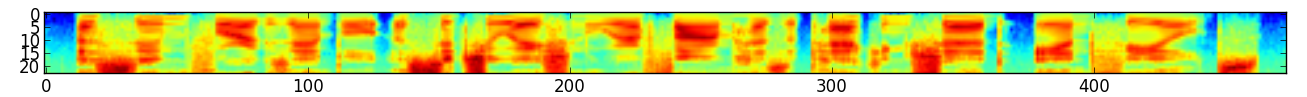
\includegraphics[width=1.0\linewidth]{../png/timitInput}
\caption{Frequency Bank input computed from a sentence contained in the \textit{TIMIT} dataset. Time is shown on x and Frequency on the y-Axis.}
\label{fig:timitInput}
\end{figure}
Filter-banks are collections of filters. These filters can be spread out over audible frequencies\footnote{Approximately 16 to 16000 Hz.}. Filter-bank output is commonly used as input for speech analysis \cite{Huang2001}\cite{Chan2015}. The number of filter-banks depends on the required resolution, 32 is a common choice \cite{Juang1987}. The energy within the part of the signal spectrum described by all individual filters is measured. Figure~\ref{fig:timitInput} shows the resulting energy measurements using 23 filters, for a sentence recording contained in the \textit{TIMIT} data set. 
The general argument for filter banks in speech recognition is that the cochlea, in the human ear, resembles a filter bank \cite[page 30]{Huang2001}. Humans do not perceive frequency linearly. Experimental evidence suggests, that our perception of is scaled according to the Mel-Scale \cite[page 34]{Huang2001}:
\begin{equation}
B(f) = 1125 ln(1 + f / 700)
\end{equation}
A normalized plot of this function is shown in figure~\ref{fig:mel} on the left.
According to the Mel-scale, humans are able to distinguish more lower frequencies than higher frequencies. In the plot the first four thousand Herz occupy roughly eighty percent of the scale. The band from four thousand to eight thousand Herz is left with only about twenty percent of the scale, even tough half of the considered frequencies are in this band. 
\begin{figure}
\centering
\includestandalone[width=6cm]{../tikz/melScale}
\includestandalone[width=6cm]{../tikz/melBank}
\caption{The Mel-scale (blue) with Mel-Frequency Cepstrum Coefficients (red)  on the left. Filterbank with Mel-spaced filters (right).}
\label{fig:mel}
\end{figure}
Mel spaced filter-banks are an attempt to include the human perception in speech recognition. The filter functions are defined by \cite[page 317]{Huang2001}:
\begin{align}
H_m &= 0 									   &\text{if}\;\; & k < f[m-1] \\
H_m &= \frac{k      - f[m-1] }{f[m] - f[m-1]}  &\text{if}\;\; & f[m-1] \leq k \leq f[m] \\
H_m &= \frac{f[m+1] - k      }{f[m + 1] - f[m]}&\text{if}\;\; & f[m] \leq k \leq f[m+1] \\
H_m &= 0									   &\text{if}\;\; & k > f[m+1] 
\end{align} 
In the equations above $H_m$ denotes the magnitude of filter $m$ with a total of $M$ filters. The frequency is denoted by $k$, the vector $f$ contains $M+2$ linearly spaced filter border values. These are the red stars on the left of  figure~\ref{fig:mel}. The right plot shows the triangular filter banks. These banks are spaced according to the same values. Roughly speaking using mel-filter banks means using a high filter resolution where human hearing is good and a low resolution where it is bad. \\
Mel-Frequency banks are considered high level feature inputs. When the recognition system is found to work with these, features on a lower level or even raw data could be used as input. The idea behind doing fewer preprocessing, is that the network might be able to come up with something better on its own.

\section{Neural Networks}
\subsection{Gradient descent}
The optimization process of neural networks is done based on a training data set $\{\{\mathbf{x}_1,\mathbf{t}_1\}, \dots , \{\mathbf{x}_p,\mathbf{t}_p\} \}$ \cite[page 156]{Rojas1996}. The elements of this set are the input- and output-patters $\mathbf{x}$ and $\mathbf{t}$ respectively. Ideally the network output should be the same as the desired one for all data pairs. The difference between target and current outputs is measured by the cost function\cite[page 156]{Rojas1996}:
\begin{align}
E = \frac{1}{2}\sum\limits_{i=1}^{p} \| \mathbf{o}_i - \mathbf{t}_i \|^2.
\end{align}
During the training process a local minimum of the error function $E$ is sought. At this minimum the difference between the network output $\mathbf{o}$ and the target values $\mathbf{t}$ is as small. This value might not be the smallest possible value, termination can happen at the global or a local minimum. 
After the training process has completed the network is expected to identify similarities to data seen during the training process and produce a similar output. 
In order to reach a local minimum, the gradient of the error function is needed. The key idea of gradient descent is to follow the negative gradient until a local minimum is reached. 
Neural networks can be considered as large composite functions, which are made up of elementary operations. The evaluation of the network can be written as a graph. Computations are done at each node and information travels trough the network along directed edges from node to node. In order to create a computational graph for the training process each of the output units of the network under consideration are connected to a new node which computes $\frac{1}{2}(o_{ij} - t_{ij})^2$\cite[page 157]{Rojas1996}. These new nodes in turn are connected to one more node, which sums up all error values and produces $E_i$. The process described above must be repeated for all training data pairs. One final node is added, which sums up all values $E_i$. Its output gives the value for the error function $E$ which is now in the form of a large graph.\\
Reverse mode algorithmic differentiation or back-propagation is an algorithm to compute the gradient of a graph consisting of basic elementary operations. As an example its operation is now illustrated using the function \cite[page 69]{Diehl2013}:
\begin{align}
f(x_1,x_2,x_3) = \sin(x_1 x_2) + \exp(x_1 x_2 x_3)
\label{eq:backFun}
\end{align}
This function written in terms of five elementary operations as \cite[page 70]{Diehl2013}:
\begin{align}
x_4 = x_1 x_2 \\
x_5 = sin(x_4)\\
x_6 = x_4 x_3 \\
x_7 = exp(x_6) \\
x_8 = x_5 + x_7 \\
y = x_8
\end{align}
Computing the gradient means computing the partial derivatives of $f$ with respect to all inputs. In this case this means finding:
\begin{align}
\frac{\partial f(x_1,x_2,x_3)}{\partial x_1} = x_2 (\cos(x_1 x_2) + x_3 \exp(x_1 x_2 x_3)) \\
\frac{\partial f(x_1,x_2,x_3)}{\partial x_2} = x_1 (\cos(x_1 x_2) + x_3 \exp(x_1 x_2 x_3)) \\
\frac{\partial f(x_1,x_2,x_3)}{\partial x_3} = x_1  x_2 \exp(x_1 x_2 x_3)
\end{align} 
Above the derivatives have been found by hand using the chain rule. Now these will be computed using back-propagation. Figure~\ref{fig:networkGraph} shows a graphical representation of equation~\ref{eq:backFun}. The partial derivatives needed for the backwards sweep can be found on the edges. \\
\begin{figure}
\centering
\includestandalone[width=12cm]{../tikz/gd_exampleNet}
\caption{Example funciton network with partial derivatives.}
\label{fig:networkGraph}
\includestandalone[width=12cm]{../tikz/gd_reverseSweep}
\caption{Reverse sweep.}
\label{fig:reverseSweep}
\end{figure}
The gradient is computed using a forward and backward sweep. During the forward sweep the inputs are fed into the network and the functions at each node are evaluated layer by layer, until the output at the last node is known. In figure~\ref{fig:networkGraph} this means computing $x_4$ to $x_8$. \\
After the forward sweep the gradient is found by going back trough the network from the output to each input node. Using a seed value of $1$ at the output node the lower unit values are computed by multiplying the associated partial derivative found on each edge. If a node has more then one incoming value, their sum is computed. The process is illustrated in figure~\ref{fig:reverseSweep}. At the roots of the tree the partial derivatives of the output with respect to each input can be found. Together these root values make up the gradient. 
To be able to perform the first forward sweep the network weights are initialized at random. The training data pairs are known and can be added as constants to the graph. 

\subsection{Deep Neural Networks}
\subsubsection{Stochastic gradient descent}
When training networks on very large training sets, working with the full data set to compute the current gradient becomes very inefficient. As a remedy its is good practice in machine learning to work with so called mini-batches. A mini-batch includes a random subset of the training data set. This procedure is known as randomized gradient descent. During training the stochastic process goes trough the data mini-batch by mini-batch. 

\subsection{Recurrent Neural Networks}
\begin{figure}
\centering
\includestandalone[width=9cm]{../tikz/recNet}
\caption{Rolled (left) and unrolled (right) recurrent neural net with two units.}
\label{fig:unrolledNet}
\end{figure}
When processing speech its is important to take context into account. When spelling the letters which make up a word, it is important to know what the previous letter was, in order to make the right decision. 
Feed-forward neural nets do not possess memory. These networks make decisions, starting from zero every time. In oder to fix this a cell state variable can be introduced. This state is fed back into the cell together with new inputs every time step. Such a layout is shown in figure~\ref{fig:unrolledNet} on the left. 
Another way to depict the same network is to not only consider the spacial dimension, but add the time axis as well. Figures, which show the spacial and time dimension are called unrolled network diagrams, shown in figure~\ref{fig:unrolledNet} on the right. The unrolled form shows a direct dependency of the output at time $t$ on the previous output at $t-1$. This causes $y_t$ and $y_{t-1}$ to change together. Or in other words: The introduction of recurrent connections leads to correlation of the two outputs. 


\subsubsection{The exploding and vanishing gradient problem}
Even tough past information is available in theory, learning long time dependencies is problematic with classical neural nets. Due to problems with gradient descent on correlated data, the back-propagated derivative can sometimes become waker and weaker until it ultimately vanishes \cite{Hochreiter1998}. Another problem is that sometimes classical recurrent neural nets produce a gradient that blows up \cite{Pascanu2012}. The exploding gradients can be fixed by clipping, but vanishing gradients require more sophisticated treatment \cite{Bengio1993}.     

\subsubsection{Long short-term memory}
Research seemed to be focused on solving the problem by making changes to the back-propagation algorithm. However a good solution to the problem turned out to
be changing the network instead. Long short-term memory (LSTM) cells as proposed in \cite{Hochreiter1995} are more complex network units.
These cells use the equation system \cite[page 5]{Graves2013}\footnote{ Various versions of LSTM cells exist. This one is commonly referred to as the \textquotedblleft peephole\textquotedblright $ \: $ variant. }:
\begin{align}
\mathbf{i_t} &= \sigma (\mathbf{W}_{ix} \mathbf{x}_t + \mathbf{W}_{ih} \mathbf{h_{t-1}} + \mathbf{W}_{ic} \mathbf{c_{t-1}} +\mathbf{ b}_i) \\
\mathbf{f_t} &= \sigma (\mathbf{W}_{fx} \mathbf{x}_t + \mathbf{W}_{fh} \mathbf{h_{t-1}} + \mathbf{W}_{fc} \mathbf{c_{t-1}} +\mathbf{ b}_f) \\
\mathbf{c_t} &= \mathbf{f_t} \mathbf{c_{t-1}} + \mathbf{i_t} \tanh( \mathbf{W}_{cx} \mathbf{x}_t + \mathbf{W}_{ch} \mathbf{h_{t-1}} + \mathbf{b}_c ) \\
\mathbf{o_t} &= \sigma (\mathbf{W}_{ox} \mathbf{x}_t + \mathbf{W}_{oh} \mathbf{h_{t-1}} + \mathbf{W}_{oc} \mathbf{c_t} + \mathbf{b}_o ) \\
\mathbf{h_t} &= \mathbf{o}_t \tanh(\mathbf{c}_t) \\
\end{align}
From the definition of the matrix product follows that
\begin{equation}
\mathbf{A}\mathbf{x}_1 + \mathbf{B}\mathbf{x}_2
=
\begin{bmatrix} \mathbf{A} & \mathbf{B} \end{bmatrix} \cdot
\begin{bmatrix} \mathbf{x}_1 \\ \mathbf{x}_2 \end{bmatrix}.
\end{equation}
Which this relation in mind the equations above can be rewritten, by creating column wise concatenated weight matrices for every neuron gate $W_i$, $W_f$, $W_o$, as well as for the state $W_c$. These matrices can then be multiplied by a row wise concatenated vector $[\mathbf{x}_t \; \mathbf{h_{t-1}} \; \mathbf{c}]^T$, which leads to the slightly simplified system of equations below:
\begin{align}
\mathbf{i_t} &= \sigma (\mathbf{W}_i [\mathbf{x}_t \; \mathbf{h_{t-1}} \; \mathbf{c_{t-1}}]^T + \mathbf{b}_i) \\
\mathbf{f_t} &= \sigma (\mathbf{W}_f [\mathbf{x}_t \; \mathbf{h_{t-1}} \; \mathbf{c_{t-1}}]^T + \mathbf{b}_f) \\
\mathbf{c_t} &= \mathbf{f}_t \mathbf{c_{t-1}} + \mathbf{i}_t \tanh( \mathbf{W}_c [\mathbf{x}_t \; \mathbf{h_{t-1}}]^T + \mathbf{b}_c ) \\
\mathbf{o_t} &= \sigma (\mathbf{W}_o [\mathbf{x}_t \; \mathbf{h_{t-1}} \; \mathbf{c_t}]^T + \mathbf{b}_o ) \\
\mathbf{h_t} &= \mathbf{o_t} \tanh(\mathbf{c_t})
\end{align}
\begin{figure}
\includestandalone[width=\textwidth]{../tikz/lstm}
\caption{Visualization of the LSTM architecture.}
\label{fig:lstm}
\end{figure}
This system of equations is visualized in figure~\ref{fig:lstm}. The diagram is read from bottom to top. The most important part is the line from $\mathbf{c}_{t-1}$ to $\mathbf{c}_{t}$ \cite{Colah2015}. It records operations on the cell state $\mathbf{c_t}$. The cell state contains information from the past which helps the block make decisions regarding the current output $\mathbf{h}_t$. The sigmoid functions $\sigma(\cdot)$ are applied element wise on the input vectors and produce outputs between zero and one. In the case of the forget gate output $\mathbf{f}_t$ these values $\in (0,1)$ well serve as a measure of how much of the past state the cell would like to remember. One means keep this variable and zero throw it away \cite{Colah2015}. 
The following task is to determine what should be added to the memory. This information can be found in the input gate result $\mathbf{i}_t$. $\mathbf{i}_t$ is multiplied element wise with the candidate values $\mathbf{\bar{c}}_t$. These are computed by a hyperbolic tangent neuron.  The $\tanh(\cdot)$ function makes sure all vector elements are between $-1$ and $1$. The neuron computing the candidate state values $\mathbf{\bar{c}}_t$ looks at input data and the past outputs. Both are labeled $\mathbf{w}$ in figure~\ref{fig:lstm}, $\mathbf{w}$ contains all information that could possibly be included in the new state. Finally the weighted candidate values are added to what was previously stored. This operation leads to the updated memory state $\mathbf{c}_t$. 
Last but not least the new output value has to be computed, which will be a filtered version of the cell state. The decision of which and how much of each state variable will be send outside is made by output gate. It's output $\mathbf{o}_t$ is multiplied with a rescaled version of the cell state. The rescaling is done using another hyperbolic tangent, which again sets all values between minus one and one. The product of this rescaled state and the weights found in $\mathbf{o}_t$ then yields the new output $\mathbf{h}_t$. 

\subsubsection{Bidirectional Long Short Term Memory}
With the advent of LSTMs deep recurrent networks became feasible in speech recognition \cite{Graves2013b}. RNNs are always deep in time, because their hidden state depends on past inputs. To enable abstraction their structure must also be deep in space. A bidirectional LSTM layer is shown in figure~\ref{fig:blstm}. It is important to note, that linear neurons are used to compute the LSTM input as well as the outputs according to the equations \cite{Graves2013b}:
\begin{align}
\overrightarrow{\mathbf{h}}_t &= \text{LSTM}(\mathbf{W}_{\overrightarrow{\mathbf{h}}_t} [\mathbf{x}_t \; \mathbf{h}_{t-1}]^T + \mathbf{b}_{\overrightarrow{\mathbf{h}}_t}) 
\\
\overleftarrow{\mathbf{h}}_t &= \text{LSTM}(\mathbf{W}_{\overleftarrow{\mathbf{h}}_t} [\mathbf{x}_t \; \mathbf{h}_{t+1}]^T + \mathbf{b}_{\overleftarrow{\mathbf{h}}_t})
\\
\mathbf{y}_t &= \mathbf{W}_{y} [\overrightarrow{\mathbf{h}}_t \; \overleftarrow{\mathbf{h}}_t]^T + \mathbf{b}_y  
\end{align}
\begin{figure}
\centering
\includestandalone[height=7 cm]{../tikz/blstm2}
\caption{A bidirectional Long short term memory layer, according to \cite{Graves2013b} }
\label{fig:blstm}
\end{figure}
If stacked on top of each other, these bidirectional LSTM layers form a deep recurrent network. Defining $\mathbf{h}^0 = \mathbf{x}$, $\mathbf{h}^N = \mathbf{y}$ looking at time from $t = 1$ to $T$ and taking $N$ layers leads to:
\begin{align}
\overrightarrow{\mathbf{h}}_t^n &= \text{LSTM}(\mathbf{W}_{\overrightarrow{\mathbf{h}}_t}^n [\mathbf{h}_t^{n-1} \; \mathbf{h}_{t-1}^n]^T + \mathbf{b}_{\overrightarrow{\mathbf{h}}_t}^n) 
\\
\overleftarrow{\mathbf{h}}_t^n &= \text{LSTM}(\mathbf{W}_{\overleftarrow{\mathbf{h}}_t}^n [\mathbf{h}_t^{n-1} \; \mathbf{h}_{t+1}^n]^T + \mathbf{b}_{\overleftarrow{\mathbf{h}}_t}^n)
\\
\mathbf{h}_t^n &= \mathbf{W}_{y}^n [\overrightarrow{\mathbf{h}}_t \; \overleftarrow{\mathbf{h}}_t]^T + \mathbf{b}_y^n
\end{align}
In this setting each LSTM cell has access to information from before or after it. For this to work the speech sequence, which is analyzed has to be recorded completely. In this case future information is available and should be used for recognition purposes.

\section{Tensor-flow}
In this section is devoted to the toolbox, which will be used to implement the Listen Attend and spell, architecture. According to the Tensor-flow authors \cite{Agarwal2015}: 
\textquotedblleft TensorFlow is an interface for expressing machine learning algorithms, and an implementation for executing such algorithms\textquotedblright . It was released by Google in 2015 and after installation can be used from within Python or C++. 



\section{Listen, Attend and Spell}
The Listen Attend and Spell architecture (LAS) is the main Idea around which this thesis revolves. This entire section is based on \cite{Chan2015}. The las-network consists of two mayor parts, the listener and the speller. The listener is a pyramidal recurrent neural net. It accepts filter bank spectra $\mathbf{x}_n$ as inputs and produces high level output features $\mathbf{h}_m$. The speller in turn accepts the features as input and outputs distributions over Latin character sequences $\mathbf{y}_p$. An overview of the las-achrcitecture is given in figure~\ref*{fig:las}.
%If maps the input sequence to a set of vectors of fixed length. The speller then takes these
%vectors and produces an output sequence \cite{Sutskever2014}.

\subsection{The listener}
The listener shown in figure~\ref*{fig:las} on the bottom, consists of Bidirectional Long Short Term Memory RNN (BLSTM) blocks. This choice implies that only fully recorded data can be analyzed.  These blocks are arranged in a pyramidal structure, such that the time resolution is cut in half in every layer. This operation reduces the length $U$ of the high level features $\mathbf{H}$. Without this compression the following attend and spell operation has a hard time extracting the relevant information. Additionally the compression reduces the problem complexity, which speeds up the training process significantly \cite[page 4]{Chan2015}.

\subsection{Attend and spell}
The speller takes the features and produces a distribution over Latin character sequences as output. The computation of this output involves the context vector $\mathbf{c}_i$, the decoder state $\mathbf{s}_i$, the features $\mathbf{H}$ and the previous output $\mathbf{y}_i$. The index $i$ denotes time, $i-1$ is used to refer to results from the last time step. \\
These values are computed using \cite[page 4]{Chan2015}:
\begin{align}
 s_i &= \text{RNN}(\mathbf{s}_{i-1}, \mathbf{y}_{i-1}, \mathbf{c}_{i-1}) \\
 \mathbf{c}_i &= \text{AttentionContext}(\mathbf{s}_i,\mathbf{H}) \\
  P(\mathbf{y}_i|\mathbf{x}, \mathbf{y}_{<i}) &= \text{CharacterDistribution}(s_i,\textbf{c}_i)
\end{align}
The state follows from a recurrent neural net (RNN) made of a two layer LSTM.
The attention mechanism, called AttentionContext above, computes a new context vector once every time step.
This computation starts with the determination of the scalar energy $e_{i,u}$, which will be used as weight for its corresponding feature vector  $h_u$. The computation starts with two feedforward neural networks or multilayer perceptrons (MLP), $\phi$ and $\psi$ \cite[page 5]{Chan2015}:
\begin{align}
e_{i,u} = \phi(\mathbf{s}_i)^T \psi(\mathbf{h_u}) \\
\alpha_{i,u} = \frac{ \exp(e_{i,u})}{ \sum\limits_{u} \exp(e_{i,u})} \\
\mathbf{c}_i = \sum\limits_{u} \alpha_{i,u} \mathbf{h}_u
\end{align}
$\alpha$ is produced by running $\mathbf{e}$ trough a softmax function, which scales $\mathbf{e}$ such that all elements are within $(0,1)$ and add up to one. These scaled weights, can then be used to form the context vector $\mathbf{c}_i$. When the training process converges the $\alpha_i$s typically follow a distribution with sharp edges\cite[page 5]{Chan2015}. Thus it is justified to think of the alphas as a sliding window. This window contains only the currently relevant parts of the condensed input data set.

\begin{figure}
\includestandalone[width=\textwidth]{../tikz/lasArcBottomUp}
\caption{The LAS architecture \cite[page 3]{Chan2015}. BLSTM blocks are shown in red. LSTM blocks in blue and attention nets in green.}
\label{fig:las}
\end{figure}

\subsection{Training}
For end-to-end speech recognition all networks must be trained jointly. The objective is to maximize the logarithmic probability:
\begin{equation}
\max\limits_\theta \sum\limits_{i} \log P(y_i | \mathbf{x}, y_{<i};\theta).
\end{equation}
Here $y_i$ denotes the current output distribution, $x$ the input, $\theta$ the various network parameters and finally $y_{<i}$ the ground truth, which is the known true desired output.
Using the known output during training creates a situation, where the past outputs are always right. In practice however the situation will be different, as the network is going to make mistakes. As it is desired to create a robust model it is necessary to sometimes include the character distribution generated by the networks being trained.
Which leads to the objective \cite[page 5]{Chan2015}:
\begin{align}
\hat{y}_{i} = \text{CharacterDistribution}(s_i,\textbf{c}_i) \\
\max_{\theta} \sum\limits_{i} \log R(y_i|\mathbf{x},\hat{y}_{<i};\theta)
\end{align}
The novelty in comparison to the previous expression is that $\hat{y}_{<i}$ is sometimes taken from the past network outputs instead of the ground truth. An idea which Chan et al. found in \cite{Bengio2015}.

\subsection{Decoding with Beam search}
In order to generate a readable text, it is necessary to choose characters from the generated character distributions. One way to do this is to simply pick the most likely letter from each distribution. This method ignores the possibility of generating better results by also considering less likely options. Therefore a broader search trough the most likely options is considered. Unfortunately memory limitations make it impossible to search trough all possible combinations. Therefore only the $n$ most likely options are explored and the rest is disregarded. Adding the most likely options for each letter produces a tree of possible transcriptions. The different routes along this tree are called hypotheses. A score for each hypothesis can be computed, by multiplication of the probability values the las-network assigned to each branch along its path. In beam search only the m most likely hypotheses are kept. Using only las-probabilities would be equivalent to picking the most likely letter at every node. Therefore a language model is required to pick the best hypothesis. Such models can be trained on text data only. A selection can then be made according to\cite[page 6]{Chan2015}:
\begin{align}
s(\mathbf{y}|\mathbf{x}) = \frac{\log P(\mathbf{y}|\mathbf{x})}{ |\mathbf{y}|_c} + \lambda \log P_{LM}(\mathbf{y})
\end{align}
Here $P_{LM}$ denotes the weight the language model assigns to each hypothesis. And $\lambda$ is a weight factor, which determines the language model importance. 





